\section{Motivation}
When consumers purchase IoT devices for their home, whether an Amazon Echo, wireless smart scale, or Nest thermostat, they currently have no visibility into the traffic that their devices are sending across the Internet or how vulnerable their devices are to attack. IoT devices have access to some of our most personal and private information, including financial data, location, health, and behavior--data that users want to prevent from being shared with adversaries and network observers. The only visibility consumers have into the privacy of their information is what they see on the apps associated with their devices on their phones; they don't have the time or capability to closely scrutinize their outgoing data via Wireshark. Thus we present IoT Network Monitor: an intuitive and user-friendly router to which consumers can connect their devices and visualize the vulnerabilities of IoT devices in their home. 

\section{Related Work}
While the academic literature does not include publications proposing a security and privacy monitoring system for home IoT devices, we summarize the research relevant to the three features we propose in IoT Network monitor: 1) default password detection, 2) privacy analysis, and 3) anomaly detection. 

Very little academic literature directly related to the default password problem of IoT devices exists. A few papers briefly mention that the default password problem is a security threat, but no previous work proposes a potential solution. 

Literature regarding the IoT and the default password problem is most prevalent in newspaper articles and blogs. Most sources of that kind discuss the security issue of this problem and mention the threat posed by the Mirai botnet, without proposing a solution. An example of this is an article written by Brian Krebs on his security blog, Krebs on Security, where he argues that it is insufficient to only change the password on the online user interface, but rather it is imperative to also change the passwords of the open ports. Most IoT users lack the knowledge to respond to Krebs' warnings, therefore, the issue still persists.

Related research into the privacy implications of IoT systems has revealed significant privacy vulnerabilities that adversaries with passive network capabilities could exploit. For example, in ``Protecting your Daily In-Home Activity Information from a Wireless Snooping Attack'' ~\cite{srinivasan2008fats}, Srinivasan et al. present a new privacy leak in residential wireless ubiquitous computing systems: the Fingerprint and Timing-based Snooping (FATS) attack. This attack allows a WiFi eavesdropper to observe private activities in the home such as cooking, showering, toileting, and sleeping by snooping on the wireless transmissions of sensors in a home and leveraging tiered inference algorithms.

In their article, Copos, et al. present a scheme to infer when a home is occupied based on parsing packet capture files and log characteristics of the network traffic from a smart thermostat. ~\cite{coposIoT}

More recently, Apthorpe et al. ~\cite{apthorpeIoT} observed that passive network observers, such as Internet service providers, could analyze IoT network traffic and infer user/device interactions even when device communications are encrypted. This attack is especially concerning for personal medical devices. The repetitive nature of medical tests, such as daily blood sugar or blood pressure readings, generates clearly defined patterns of device activity and could reveal common medical conditions from network metadata alone. 

\section{Proposed Architecture}
As consumers continue to adopt IoT devices, they will continue to place insecure IoT devices within networks in positions of trust (e.g. smart home networks). Behind the firewall, these IoT devices will have access to other network devices and can pose a variety of security threats. For example, if the device has open ports or insecure passwords, these IoT devices can be hijacked, reveal sensitive information, conduct denial of service attacks on the local network, join an IoT botnet, etc. Yet, consumers don't have a simple, intuitive interface to understand and monitor these threats. Even if they are aware of a security attack, consumers often are not sure what action to take in response. We propose the IoT Network Monitor to help combat these issues.

Our framework for the IoT Network Monitor includes a user friendly web interface that integrates with a network middlebox that can sniff traffic on the LAN. The IoT Network Monitor collects packet captures as PCAP files throughout the day (say, for the first ten minutes of each hour). The Hub software then runs a variety of scripts to parse and analyze the latest PCAP files. It looks for vulnerabilities in the following three dimensions:

\textbf{Password Vulnerability:} Scan IoT devices on the network, looking for open ports 22 and 23, and offering a new password if the password can be cracked using brute force. 

\textbf{Privacy Analysis:} Check for unencrypted payloads in packet captures containing personal identifiers and other forms of sensitive data (e.g. medical data).

\textbf{Anomaly Detection:} Detect IoT Botnet DoS traffic originating from an IoT device on the LAN using the FITBOT framework.


\section{Implementation}
We implemented the web app as a Flask app to help integrate the front-end interface with the python scripts analyzing the network. This software, as is, is written to be deployed on a Raspberry Pi 3 and relies on the dumpcap utility for packet capture.
		
One thing to note are the challenges associated with designing the user experience with the web platform. Apart from notifying users of security threats with clear colors and relevant text (e.g. sample of leaked sensitive information or a proactive suggestions for a new password), we always provided a call to action to help users understand what to do next in response to a threat.

\begin{figure}
  \centering
    \fbox{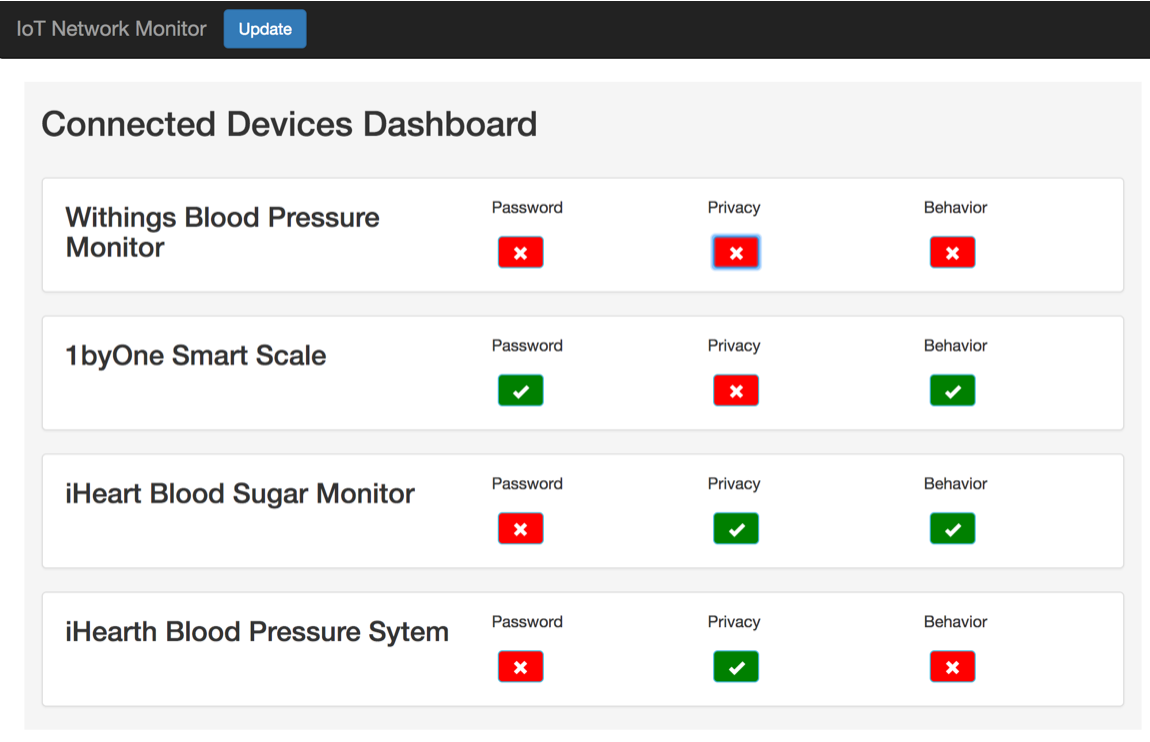
\includegraphics[scale=0.3]{ui}}
     \caption{User interface of the IoT Network Monitor}
     \label{fig:bp-image}
\end{figure}

\begin{figure}
  \centering
    \fbox{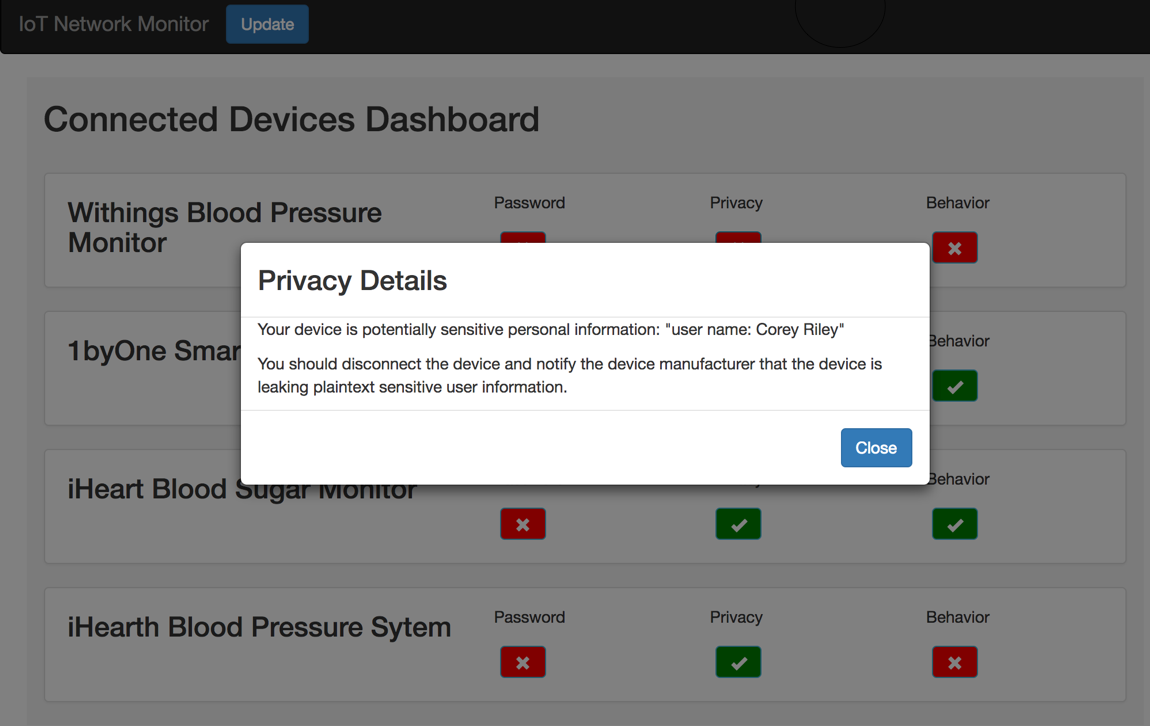
\includegraphics[scale=0.3]{alert}}
     \caption{IoT Network Monitor alerts the user when it has discovered a vulnerability}
     \label{fig:bp-image}
\end{figure}

\section{Password Inspection}
The first feature of the IoT Network Monitor scans the home network for devices that have been shipped with a default username and password combination on an open port, either port 22 or port 23 (the SSH port or the Telnet port, respectively). This vulnerability of IoT devices is created when multiple devices are shipped with the same default logon credentials, enabling the construction of the mass password attacks such as the Mirai botnet. When devices with default passwords are detected on a home network, our tool changes the password of the open port to a randomly generated 12 character string and notifies the user of the new password on the user-interface.

The implementation of the password inspection was as follows: First, Nmap, a network scanner, is used to scan the home network for all devices listening on ports 22 and 23. It scans a range of 256 IP-addresses based on the IP address of the device that the software is running on. This range should be sufficient to capture all devices on a regular home network, while still maintaining a fast runtime.

Next, The same list of 62 default logon credentials as was used in the Mirai botnet source code is then used in an attempt to log on to the devices found by Nmap. If either a SSH or a Telnet connection is successfully established, the correct username and password combination for the specific device has been found.

Once all devices with default passwords have been detected, the tool logs on to the devices using the newly found logon credentials. Then, it uses the bash-command \textit{passwd} to change the password to a randomly generated string, consisting of 12 characters that can be upper or lower case ASCII-characters and digits 0-9.

Lastly, when vulnerable devices are detected, the new randomly generated password is returned to the user on the user-interface of the IoT network monitor. However, if all 62 logon attempts to a particular device are unsuccessful, it is assumed that the device does not come with a default password, and is labeled secure on the user interface. 

\section{Privacy Analysis}
The second feature of IoT Network Monitor intercepts packet data from connected IoT devices and detects potentially sensitive information about the user that is being sent in the clear from the device to the router and on to the server. If IoT Network Monitor discovers that a device is leaking personally identifiable information or medical information, it alerts the user of this behavior. 

The feature is implemented using a six step approach. First IoT Network Monitor separates connected devices on the network into separate packet streams for analysis. This can be done by classifying packet conversations by the external IP address of the communicating with the device, since the gateway router typically makes it difficult to divide outgoing traffic into sets based on IP addresses of the origin device. 

Next, the IoT Network Monitor begins the process of deep packet inspection by separating the stream by network protocol. It separates HTTP and TCP packets for further analysis. 

After that, packet payloads are separated from the packet headers so that IoT Monitor can examine the application data and screen in for plaintext leaks. 

Packets are then classified as either plaintext or encrypted using payload entropy as an indicator of encryption. By training IoT Network Monitor on a test set of payloads, we observed a threshold entropy value below which we were able to consistently identify plaintext packets. Entropy analysis is conducted using the Shannon Entropy Test.

The test calculates the entropy of each payload string, which is a quantitative measure of the variability in the frequency of the different possible characters. While encrypted strings have very high entropy, unencrypted plaintext exhibits fairly low entropy, and is thus fairly easy to identify. This is because most characters are drawn from the limited set of printable characters and in English, many letters are much more likely to appear than others. For example, the letter e appears roughly 12.5\% of the time, while the letter $j$ appears less than 0.2\% of the time. To calculate the Shannon Entropy of a string, let $X$ be a random variable that takes on possible values $x_1$, $x_2$, ..., $x_n$. $p(x_i)$ is the probability that $X = x_i$:
$$H(X) = - \sum_{i = 1}^{n} p(x_i) log p(x_i)$$
A packet's payload is assumed to be unencrypted if its Shannon entropy value is lower than a threshold parameter. We used a relatively high threshold parameter of $7.5$, so as not to discard any unencrypted payloads with high entropy (at the cost of misidentifying a small number of encrypted payloads with low entropy).

Plaintext packets which have been identified are further analyzed for potentially sensitive information. This is implemented by a straightforward dictionary search; plaintext packets are searched for the presence of common first names, medical terms, and personally identifying information. If the monitor discovers instances of these terms in the unencrypted packets coming from an IoT device, it alerts the user on the Connected Devices Dashboard.

Lastly, in cases when devices encrypted application-level data or utilized secure protocols such as TLS or SSL, we were still able to infer rough user behavior during traffic collection due to the fact that the devices studied are only used to make periodic measurements and are not always on. For example, blood sugar may be measured at regular intervals throughout the day (such as after a meal) and smart scales might be used once every morning. Using Wireshark, we were able to associate periods of device activity based on time stamps and origin IP addresses, thereby keeping track of each device reading. In some cases, we were able to determine what the behavior of the user during that period of activity by examining the descriptions of the destination IP addresses in Wireshark.

\section{Anomaly Detection} 
The third feature of IoT Network Monitor is a feature that detects anomalous behavior of any devices connected to the hub. Many IoT devices are fundamentally insecure, exposing the Internet to a variety of new attacks.~\cite{apthorpeIoT} In particular, IoT botnets, like the Mirai botnet, are leveraging these insecure IoT devices to conduct some of the strongest distributed denial of service (DDoS) attacks ever recorded. These type of IoT botnet attacks are growing in frequency and magnitude, restricting the ability of citizens to access the Internet freely and reliably.
This has spurred interest in developing network mechanisms, particularly at the local level, for detecting attack traffic from compromised IoT devices.~\cite{AnomalyDetectionSurvey} The key challenge lies in determining which features capture the unique statistical properties of IoT traffic and help differentiate it from anomalous IoT attack traffic. After all, IoT traffic has many unique behaviors which can be leveraged to enhance machine learning accuracy.

We propose FITBOT (Find IoT Botnets), a novel packet-level machine learning anomaly detection framework for detecting botnet attack traffic in consumer Internet of Things (IoT) device networks. The key contributions in feature engineering leverage observations of IoT-specific device behaviors (e.g. limited number of endpoints, regular internal time intervals between packets, small size packet payloads for attacks, etc.).

The FITBOT framework proposes four key steps:

\textbf{Network Packet Capture:} The middlebox will sample network traffic and generate a packet capture files (PCAP) that contains a variety of flow-based attributes; no deep-packet inspection is required. For each packet, we record the following flow-based attributes: source IP address, source port, destination IP address, destination port, packet size in bytes, and the time elapsed since the last packet arrived. 

\textbf{Split Packet By Device and Time-bin:} In order to generate temporal features on a per-device basis, the packets must be split by their source IP address. This way, we can quantify and represent whether specific devices are behaving anomalously in a given time period. Using the timestamps of the packet capture, we split packets into continuous non-overlapping time-bins. The length of the time-bin may be modified to capture different types of temporal features. 

\textbf{Generate Feature Vectors for Each Packet:} We generate packet-level features and temporal features for each packet and concatenate all these features into a feature vector. Packet-level features are normally derived almost directly from the flow-based attributes; this includes packet length, interpacket timing velocity and acceleration, and protocol. Temporal-based features include bandwidth and count of distinct destination IP addresses within a given time window.

\textbf{Binary Classification:} We formulate this anomaly detection problem as a classified binary classification task. A variety of classifiers, such as Support Vector Machines, K-Nearest-Neighbors, Random Forests, and Decision Trees, can be used at this step to output a final packet-level prediction.

A key advantage of our framework is that it is flow-based, stateless, and protocol-agnostic; therefore, it can be implemented on most types of LAN middleboxes (e.g. routers, network switches, firewalls).

\section{Evaluation}

We created an isolated test environment where we could connect various medical IoT devices to a network and capture live traffic. We configured a Raspberry Pi 3 as a Wi-Fi access point (AP) and programmed it to record traffic to and from connected Wi-Fi stations (Figure~\ref{fig:data-collection}).  Creating an isolated test environment was necessary because it enabled us to easily separate traffic by device and filter out extraneous traffic on the network. We chose six IoT devices to inspect, including a Nest Smart Camera, WeMo Smart Switch, and Withings Wireless Blood Pressure Monitor.

%\begin{figure}
  %\centering
   % \fbox{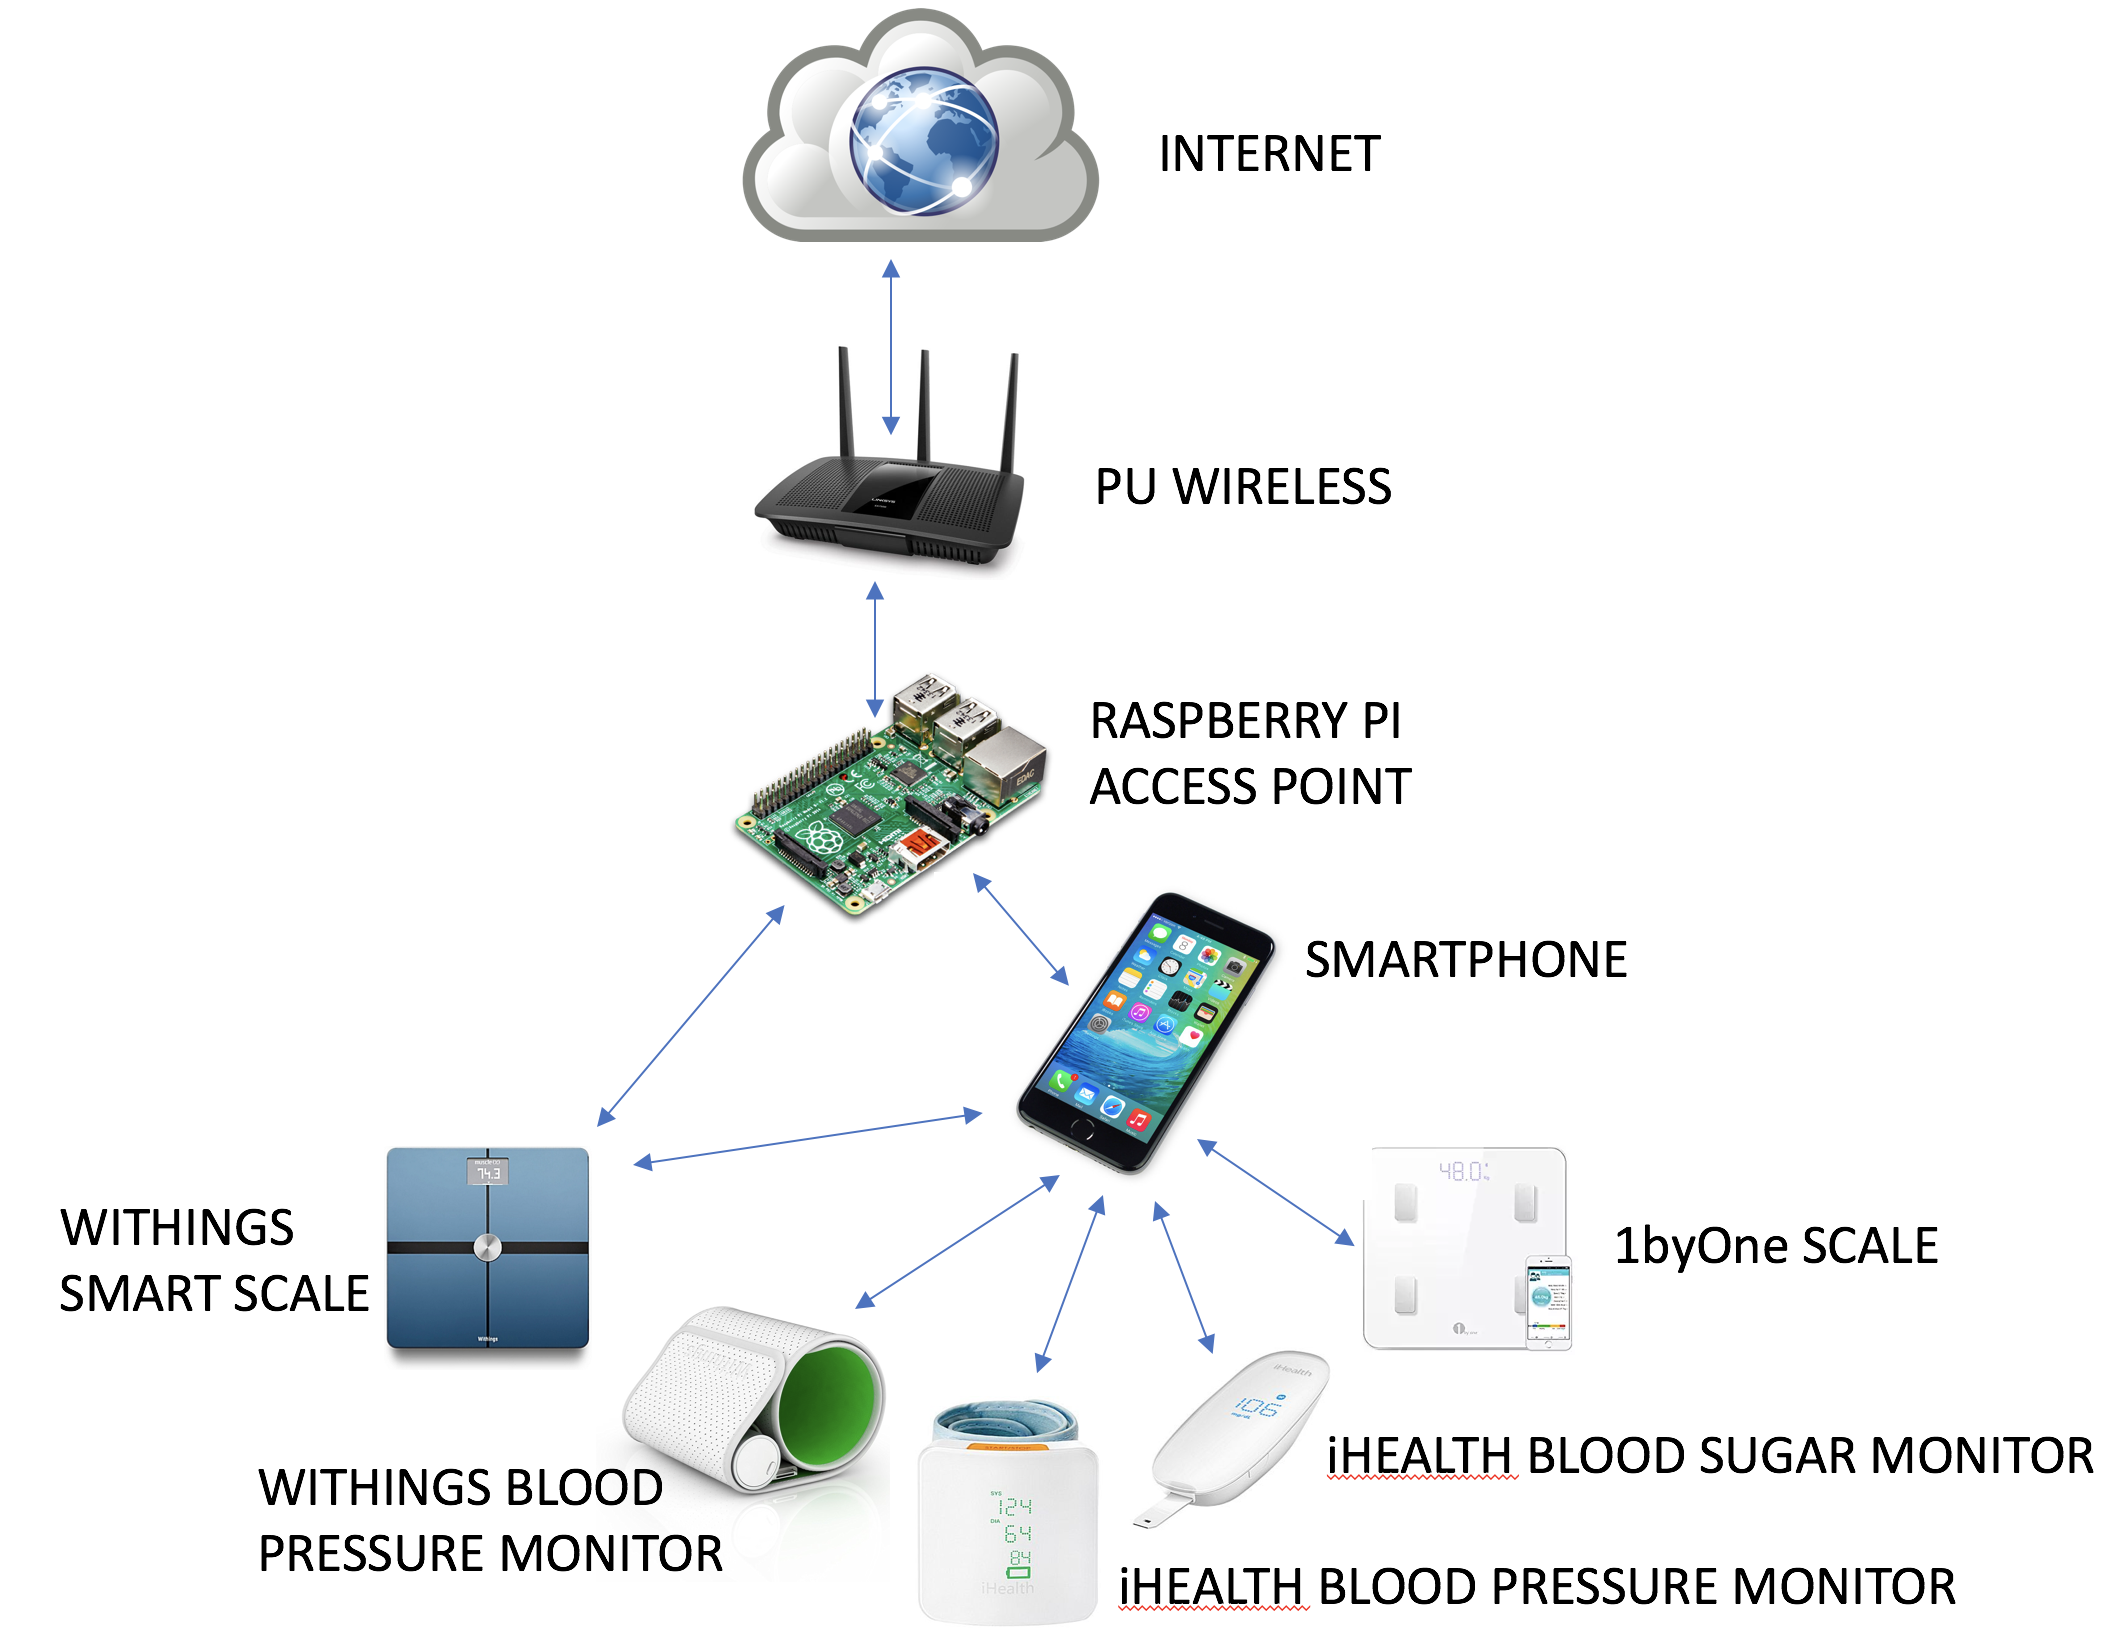
\includegraphics[scale=0.15]{network}}
  %\caption{Data collection environment and connection patterns between devices and infrastructure components.}
  %\label{fig:data-collection}
%\end{figure}

\subsection{Password Detection}
% Evaluation and testing of the project during the implementation stage was conducted using a Raspberry Pi v3. A small local network was set up to make it convenient to keep track of the devices that were connected to the network. During implementation, the code scanned a specific IP-range (172.24.1.0/24), which included the IP-address of the Pi. On the Raspberry Pi, it was possible to change which ports were open and change the password of the device as desired, in order to readily test the functionality of the code and make the debugging process easier. This allowed for a controlled testing environment.

The IoT Network Monitor was successfully able to identify the devices on the specified IP range on the network. Furthermore, after finding which devices had a default username and password combination, the code successfully changed the password from the default one to a random twelve character string. It successfully did so, both for devices with an open Telnet port, as well as for devices with an open SSH port. Then, it returned information about the device (its IP-address, port number, default logon credentials, and the new password) to the user.
\par
The code returns a JSON object when a default username and password combination is detected on a device. An example of an output from a device with IP-address 172.24.1.1 and an open SSH port
with default username \textit{root} and default password \textit{password} that gets changed to the random string \textit{sTBM9JFbgXjU} is the following:
\par
[{``172.24.1.1'': {``defaultUsr'': ``root'', ``newPass'': ``sTBM9JFbgXjU'', ``defaultPass'': ``password'',
``port'': 22}}]
\par
From this, we extract the new password (in this case \textit{sTBM9JFbgXjU}) and display it for the user on the dashboard of the IoT Network Monitor. Since the password has already been changed, the user does not need to worry about which port was insecure, or what the default username is. The value of the new password is sufficient to ensure the security of the device with regards to the default password problem.

\subsection{Privacy Analysis}
We found a very large variability in the methods each device used to send application data through the network when registering users, sending patches and updates, measuring vitals, or retrieving health analytics. All of the devices used encryption and protocols such as TLS or SSH to send sensitive first order information, such as the user's actual weight or blood sugar levels. However, there were various degrees of leaking second order information and metadata, scraped from sources such as HTTP GET requests, packet header information, and device conversation IP tables.

\begin{figure}
  \centering
    \fbox{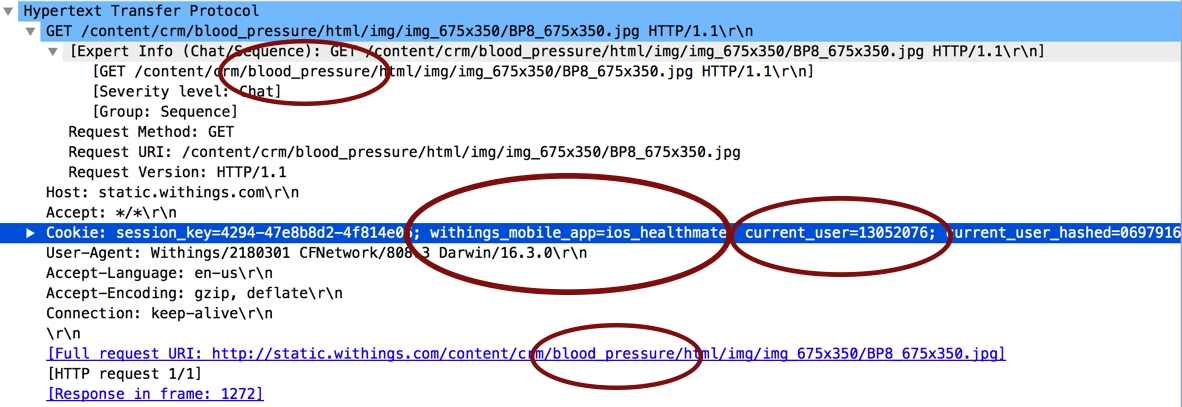
\includegraphics[scale=0.3]{bloodpacket}}
  \caption{HTTP packet sent by IoT blood pressure monitor reveals nature of device and user behavior.}
  \label{fig:bp-packet}
\end{figure}

Out of the devices that we studied, the Withings Blood Pressure Monitor exhibited the most number of vulnerabilities when it comes to revealing sensitive user information during data transmission. Figure 4 highlights the example of one packet alone, which revealed four sources of valuable information about the device. The plaintext string ``blood\textunderscore pressure'' appears twice, along with the string ``withings\textunderscore mobile\textunderscore app=ios\textunderscore healthmate''. Lastly, the ``current\textunderscore user'' field, while not directly disclosing the name of user, is potentially a unique identifier that associates that user with the subsequent blood pressure data. By monitoring this traffic for a period of time with many users, it would be trivial to match each packet of transmitted application data to the associated user. 

\subsection{Anomaly Detection}

We experimentally generate normal and attack network traffic on a simulated consumer IoT device network. Over a ten minute window, we have our IoT devices toggle through its different network states for normal traffic. And, for attack traffic, each device periodically conducts each of the three most common classes of DoS attacks associated with Mirai-infected devices: TCP SYN Flood, a UDP Flood, and a HTTP GET Flood.

By applying our framework on the local router, we identify normal and attack traffic with an accuracy above 99\%; we found that random forest and K-Nearest-Neighbors classifiers were particularly effective, outperforming decision trees and support vector machines. A feature importance analysis reveals that packet-level features greatly outperform temporal features. The differences in the distributions between normal and attack traffic were relatively more statistically pronounced, a difference which the ML algorithms were able to leverage to enhance classification performance. This is good news because the packet-level features are more lightweight in the first place since they are fully stateless and derived from network-flow attributes (e.g. 5-tuple and packet size). 

Still, the temporal features help capture and leverage IoT-specific traffic behaviors that were responsible for a classification performance boost. All of the classifiers we examined experienced approximately a .02 boost in F1 score by leveraging these features. Thus, by adding features to represent per device send/receive rates and the change in number of endpoints, we were able to leverage IoT-specific behaviors to enhance our anomaly detection framework.

\section{Conclusions}
Along with the quality of the framework, we put specific emphasis on the user-friendliness of the proposed IoT Network Inspector. As we envision regular homeowners adapting this product, many of which are not very tech-savvy, it was very important to us that the user-interface would be implemented in a straightforward and an intuitive way. To allow for a wide adoption of a product such as this one, it is vital that the product is easy to use and can provide homeowners a clear and a simple view of the security of their home network.
We believe that the three features that the IoT Network Monitor focuses on are the foundational factors of a secure smart-home. By allowing users to easily monitor the security of sensitive personal information being sent by their devices, the likelihood of cyberattacks (such as ransom attacks) on users of IoT devices would decrease. 

Furthermore, more pressure would be put on manufacturers as more users would discontinue the use of vulnerable devices, forcing manufacturers to take action and ensure proper encryption. Moreover, as this tool changes default passwords of devices, a wide adoption of this device would disable the construction of Mirai based botnets, therefore, eliminating some large DDoS attacks. However, if it so happens that a device on a home network does become a part of a botnet, our tool will advise the user to disconnect the device and discontinue its usage, further decreasing the risks of large attacks of such kind. Therefore, a wide adoption of this device would not only increase the security of specific homes, but get us much closer to a more secure worldwide IoT network.

\section{Future Work}
After completion, this project was presented at the 23rd Annual Capitol Hill Exhibition in Washington D.C., held by the Coalition for National Science Funding (CNSF). At the exhibition, we demonstrated our IoT Network monitor for attendees, including members of Congress, France C�rdova (the NSF Director), Jim Kurose (Assistant Director of CISE), and Rush Holt (former Congressman and the current President of AAAS). The IoT Network Monitor was very well received by the audience, that engaged with us in very interesting conversations about our tool, security regarding IoT devices, and information security in general.\footnote{See Bryan Mosley's blog post on the exhibition: http://cra.org/crn/2017/06/nsf-funded-iot-security-research-excites-attendees-2017-cnsf-exhibition/}
\par
Moreover, we submitted the IoT Network Monitor as an entry to the IoT Home Inspector Challenge held by the Federal Trade Commission. In the fall of 2017 we plan on collaborating with our professor, Dr. Nick Feamster, in an attempt to publish an academic paper on this project.

